


\subsection{Liquidity And Reserves Management: Strategies And Policies Ch5}



\subsubsection{The demand - supply framework}

\begin{itemize}
\item Five sources of fund demand
    \begin{itemize}
    \item Customers withdrawing money from their accounts
    \item Credit requests from customers
    \item Repayment of borrowings
    \item Other operating expenses
    \item Dividend payment to shareholders
    \end{itemize}
\item Five sources of fund supply
    \begin{itemize}
    \item New customer deposits: the most important source
    \item Customers repaying their loans
    \item Sales of assets
    \item Selling non deposit services
    \item Borrowings in the money market
    \end{itemize}
\item Net liquidity position ($L_t$)
    \begin{itemize}
    \item $L_t$ = Supplies of liquidity - Demands of liquidity
        \begin{itemize}
        \item $L_t$< 0: Liquidity deficit
        \item $L_t$> 0: Liquidity surplus
        \end{itemize}

        \begin{figure}[H]
            \centering
            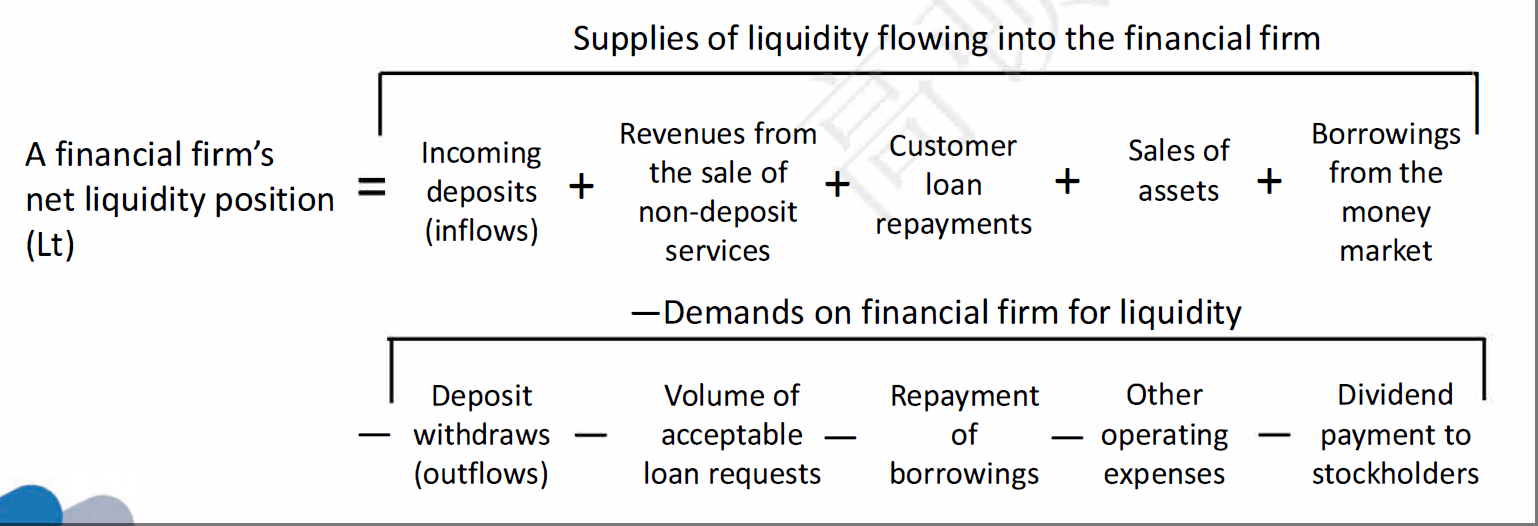
\includegraphics[width=0.5\textwidth]{images/net.png}
            \caption{net}
            \label{fig:labe22}
            \end{figure}
    
    \end{itemize}
\item Examples
    \begin{itemize}
    \item Over the next 24 hours, ABC Bank estimates that the following cash inflows and outflows (all figures in millions) will occur. What is the bank's projected net liquidity position?
    
    \begin{tabular}{@{}lc@{}}
        \toprule
        Deposit withdrawals & \$35 \\
        Deposit inflows & \$20 \\
        Scheduled loan repayments & \$50 \\
        Acceptable loan requests & \$60 \\
        Borrowing from the money market & \$38 \\
        Sales of bank assets & \$90 \\
        Stockholder dividend payments & \$10 \\
        Revenues from sale of non - deposit services & \$22 \\
        Repayment of bank borrowings & \$30 \\
        Operating expenses & \$15 \\
        \bottomrule
        \end{tabular}
    \item Answer:
        \begin{itemize}
        \item Supplies of liquidity= 20 + 50 + 38 + 90 + 22 = 220
        \item Demands of liquidity= 35 + 60 + 10 + 30 + 15 = 150
        \item Net liquidity position = Supplies of liquidity - Demands of liquidity = 220 - 150 = 70 million dollars.
        \end{itemize}
    \end{itemize}
\end{itemize}




\subsubsection{Strategies for liquidity management}

\begin{itemize}
    \item \textbf{Asset liquidity management strategies (Asset conversion strategies)}
      \begin{itemize}
        \item \textbf{Definition:} Store liquidity in assets, mainly cash and marketable securities.
        \item \textbf{Main users:} Smaller financial institutions.
        \item \textbf{Pros:} Less risky than relying on borrowings.
        \item \textbf{Cons:} High opportunity cost, as investing in liquid assets means forgoing higher returns on other assets.
      \end{itemize}
    \item \textbf{Borrowed liquidity management strategies (Liability management strategies / Purchased liquidity strategies)}
      \begin{itemize}
        \item \textbf{Definition:} Raise liquid funds through borrowings in the money market.
        \item \textbf{Purest form:} Borrow immediately spendable funds to cover all anticipated demands for liquidity.
        \item \textbf{Main users:} Largest banks.
        \item \textbf{Pros:}
          \begin{itemize}
            \item Lowering opportunity cost.
            \item Leave assets portfolio unchanged, higher expected return.
            \item Offer different rates to meet different funds needed.
          \end{itemize}
        \item \textbf{Cons:} Most risky approach due to volatility of interest rates and rapid changes in credit availability.
      \end{itemize}
      \item \textbf{Balanced liquidity management strategies}
      \begin{itemize}
        \item \textbf{Definition:} expected liquidity demands are stored in assets (marketable securities) and advance arrangements for lines of credit. Unexpected cash needs are met by near-term borrowings.
        
        \item \textbf{Pros:Strike a balance between risk and opportunity cost.}
      
      \end{itemize}
  \end{itemize}


  \subsubsection*{Estimating liquidity needs}

  \begin{itemize}
    \item :Sources and uses of funds approach
    
    Estimated liquidity deficit(-) or surplus \((+)\) for the coming period:
    
    \(=\) Estimated change in deposits \(-\) Estimated change in loans
    \item Estimating future deposits and loans divides the forecast of future deposit and loan growth into three components:
      \begin{itemize}
        \item A trend component
        \item A seasonal component
        \item A cyclical component
      \end{itemize}
    \item \textbf{Example}
      \begin{itemize}
        \item Forecasting deposits and loans with the sources and uses of funds approach (figures in millions of dollars)
          \begin{center}
          \adjustbox{max width=\textwidth}{
          \begin{tabular}{|p{3cm}|p{3cm}|p{3cm}|p{3cm}|p{3cm}|}
          \hline
          Deposit Forecast for Deposits & Trend Estimate for Deposits & Seasonal Element & Cyclical Elements & Estimated Total Deposits \\
          \cline{1-5}
          January, Week 1 & \$1,210 & -4 & -6 & \$1,200 \\
          January, Week 2 & 1,212 & -54 & -58 & 1,100 \\
          January, Week 3 & 1,214 & -121 & -93 & 1,000 \\
          January, Week 4 & 1,216 & -165 & -101 & 950 \\
          February, Week 1 & 1,218 & +70 & -38 & 1,250 \\
          February, Week 2 & 1,220 & +32 & -52 & 1,200 \\
          \hline
          \end{tabular}
          }
          \end{center}
        \item Forecasting deposits and loans with the sources and uses of funds approach (figures in millions of dollars)
          \begin{center}
          \adjustbox{max width=\textwidth}{
            \begin{tabular}{|p{3cm}|p{3cm}|p{3cm}|p{3cm}|p{3cm}|}
                \hline
          Loan Forecast for Loans & Trend Estimate for Loans & Seasonal Element & Cyclical Elements & Estimated Total Loans \\
          \cline{1-5}
          January, Week 1 & \$799 & +6 & -5 & \$800 \\
          January, Week 2 & 800 & +59 & -9 & 850 \\
          January, Week 3 & 801 & +174 & -25 & 950 \\
          January, Week 4 & 802 & +166 & +32 & 1,000 \\
          February, Week 1 & 803 & +27 & -80 & 750 \\
          February, Week 2 & 804 & +98 & -2 & 900 \\
          \hline
          \end{tabular}
          }
          \end{center}
        \item Forecasting liquidity deficits and surpluses with the sources and uses of funds approach (figures in millions of dollars)
          \begin{center}
          \adjustbox{max width=\textwidth}{
          \begin{tabular}{|p{3cm}|p{2.4cm}|p{2.4cm}|p{2.4cm}|p{2.4cm}|p{2.4cm}|}
          \hline
          Time Period & Estimated Total Deposits & Estimated Total Loans & Estimated Deposit Change & Estimated Loan Change & Estimated Liquidity Deficit (-) or Surplus (+) \\
          \cline{1-6}
          January, Week 1 & \$1,200 & \$800 &  &  &  \\
          January, Week 2 & 1,100 & 850 & -100 & +50 & -150 \\
          January, Week 3 & 1,000 & 950 & -100 & +100 & -200 \\
          January, Week 4 & 950 & 1,000 & -50 & +50 & -100 \\
          February, Week 1 & 1,250 & 750 & +300 & -250 & +550 \\
          February, Week 2 & 1,200 & 900 & -50 & +150 & -200 \\
          \hline
          \end{tabular}
          }
          \end{center}
      \end{itemize}
  \end{itemize}
  
  \subsubsection{Estimating liquidity needs}
  \begin{itemize}
    \item The structure of funds approach
        \begin{itemize}
            \item Total liquidity requirement \(=\) Deposit and nondeposit liability liquidity requirement + loan liquidity requirement 
            \item Deposit and non-deposit liability liquidity requirement: deposits and other funds are divided into categories based upon their estimated probability of being withdrawn:
            \begin{itemize}
                \item "Hot Money" liabilities (volatile liabilities)
                \item Vulnerable funds
                \item Stable funds (core deposits or core liabilities)
                \item Liability liquidity reserve calculation:  \(0.95 \times\) (Hot money deposits and nondeposit funds - Required legal reserve) \(+ 0.30 \times\) (Vulnerable deposit and nondeposit funds - Required legal reserve) \(+ 0.15 \times\) (Stable deposits and nondeposit funds - Required legal reserve)
            \end{itemize}
            \item Loan liquidity requirement:
            \begin{itemize}
              \item 100\% satisfy customers needs.
              \item loan liquidity requirement \(= 1.00 \times\) (Potential loans outstanding - Actual loans outstanding)
            \end{itemize}

        \end{itemize}
    
       
      \end{itemize}

  
  







\subsubsection{Example: The structure of funds approach}

\begin{itemize}
  \item New Bank finds that its current deposits and non-deposit liabilities break down as follows:
  \begin{itemize}
    \item Hot money: 30 million (95\% liquidity reserve portion)
    \item Vulnerable funds: 25 million (30\% liquidity reserve portion)
    \item Stable (core) funds: 120 million (15\% liquidity reserve portion)
  \end{itemize}
  \item Each kind of deposit has a required 3\% legal reserve by the central bank. The bank's total loans requirement recently are likely to be \$160 million from \$145 million actual loans. This financial firm decides to be ready to honor customer demands for all loans that meet its quality standards. What is the bank's total liquidity requirement?
  \item \textbf{Answer:}
    \[
    \begin{aligned}
        &\text{Total liquidity requirement calculation} \\
        =&
      0.95 \times (30 - 0.03 \times 30)  + 0.30 \times (25 - 0.03 \times 25) + 0.15 \times (120 - 0.03 \times 120) + 100\% \times (160 - 145) \\
      =& 67.38\ \text{million}
    \end{aligned}
    \]

\end{itemize}







\subsubsection{Estimating liquidity needs}
\begin{itemize}

\item The structure of funds approach
    \begin{itemize}

    \item Refine the structure of funds approach by calculating expected liquidity requirements based on probabilities of different possible outcomes.
   
    \end{itemize}
\[
    \begin{aligned}
        \text{Expected liquidity requirement} &= \text{Probability of Outcome A} \times (\text{Estimated liquidity surplus or deficit in Outcome A}) \\
        &+ \text{Probability of Outcome B} \times (\text{Estimated liquidity surplus or deficit in Outcome B}) \\
        &+ \cdots + \cdots
        \end{aligned} \]
\end{itemize}





\subsubsection{Example: refine the structure of funds approach}



\begin{center}
\adjustbox{max width=\textwidth}{
\begin{tabular}{|p{3cm}|p{3cm}|p{3cm}|p{3cm}|p{3cm}|}
\hline
\phantom{X} & Estimated Deposits Next Week (millions) & Estimated Loans Next Week (millions) & Estimated Liquidity Position Next Week (millions) & Probability to Each Possible Outcome \\
\cline{1-5}
Best position & 190 & 100 & +90 & 15\% \\
\cline{1-5}
Normal position & 170 & 130 & +40 & 65\% \\
\cline{1-5}
Worst position & 140 & 160 & -20 & 20\% \\
\cline{1-5}
\hline
\end{tabular}
}
\end{center}

Expected liquidity requirement = 90 × 15\% + 40 × 65\% + (-20) × 20\% = 35.5 million




\subsubsection{Estimating liquidity needs}

\begin{itemize}
\item Liquidity indicator approach
    \begin{itemize}
    \item Many financial-service institutions estimate their liquidity needs based upon experience and industry averages, which means using certain liquidity indicators.
    
   
    \begin{table}[H]
        \centering
        \rowcolors{2}{gray!10}{white}
        \begin{tabular}{|p{3cm}|p{6.5cm}|p{6.5cm}|}
        \hline
        \rowcolor{gray!20}
        \textbf{Liquidity indicator} & \textbf{Description} & \textbf{Liquidity impact (the higher the ratio)} \\ \hline
        Cash position indicator & Cash and deposits from depository institutions / Total assets & The smaller the chance of a liquidity crisis \\
        Core deposit ratio & Core deposits / Total assets & The smaller the chance of a liquidity crisis \\
        Deposit composition ratio & Demand deposits / Time deposits & The greater the chance of a liquidity crisis \\
        Deposit brokerage index & Brokered deposits / Total deposits & The greater the chance of a liquidity crisis \\ \hline
        Liquid securities indicator & U.S.\ gov.\ securities / Total assets & The smaller the chance of a liquidity crisis \\
        Pledged securities ratio & Pledged securities / Total securities holdings & The greater the chance of a liquidity crisis \\
        Hot money ratio & Money‐market assets / Volatile liabilities & The smaller the chance of a liquidity crisis \\ \hline
        Capacity ratio & Net loans \& leases / Total assets & The greater the chance of a liquidity crisis \\
        Loan commitments ratio & Unused loan commitments / Total assets & The greater the chance of a liquidity crisis \\
        Net Fed funds \& repo position & (Fed funds sold + rev.\ repos − Fed funds purchased − repos) / Total assets & The smaller the chance of a liquidity crisis \\ \hline
        \end{tabular}
        \caption{Comprehensive Liquidity Indicators}\label{tab:liquidity-ind}
        \end{table}
    \end{itemize}
\end{itemize}





\subsubsection{Legal reserve}
\begin{itemize}
\item Lagged reserve accounting (LRA) is used to calculate Legal Reserves.
    \begin{itemize}
    \item Reserve computation period: two-week period from a Tuesday through a Monday two weeks later.
    \item Reserve maintenance period: 14-day period stretching from a Thursday through a Wednesday.
    \item Reserve funding period: reserve maintenance begins 30 days after the beginning of the reserve computation, which allows the money position manager 16 days to plan.
    \end{itemize}

    \begin{figure}[H]
        \centering
        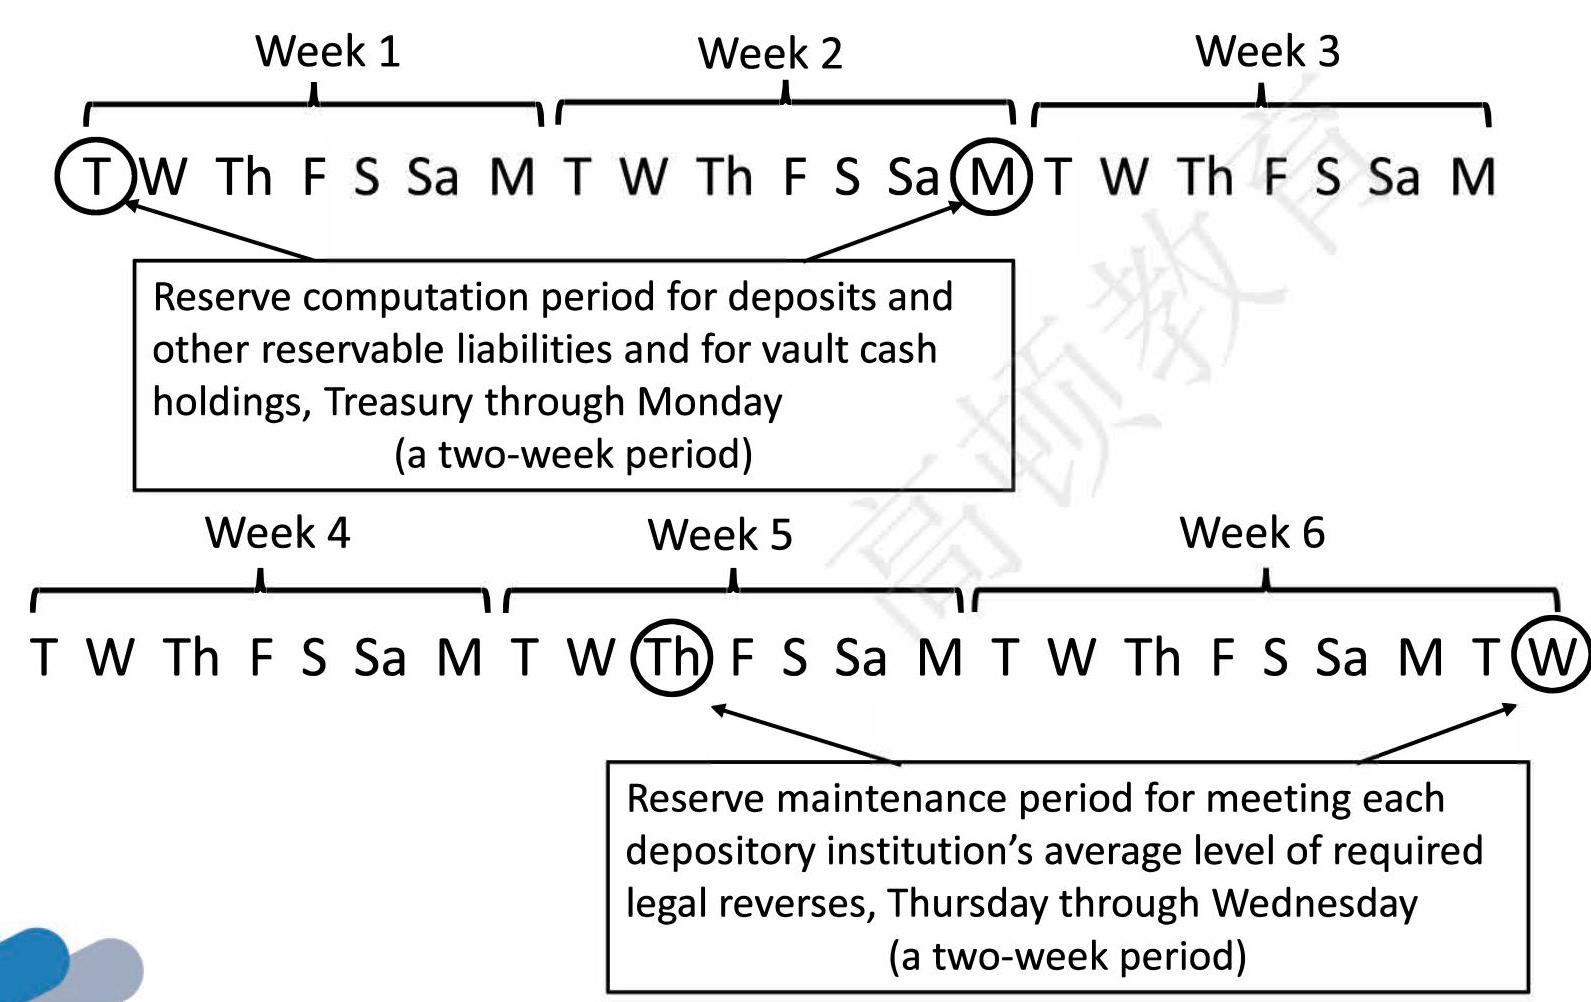
\includegraphics[width=0.5\textwidth]{images/Legal Reserves.jpg}
        \caption{Legal Reserves}
        \label{fig:labe22}
        \end{figure}

\item Total required legal reserves = Reserve requirement on transaction deposits × Daily average amount of net transaction deposits over the computation period + Reserve requirement on nontransaction reservable liabilities × Daily average amount of nontransaction reservable liabilities over the computation period
\item Alternative sources of reserves:
    \begin{itemize}
    \item Federal funds market
    \item Selling liquid securities
    \item Drawing upon any excess correspondent balances placed with other depository institutions
    \item Repo
    \item Selling new time deposits to the largest customers
    \item Borrowing in the Eurocurrency market
    \item Central bank’s discount window
    \end{itemize}
  
\item Factors in choosing among the different sources :
    \begin{itemize}
    \item Immediacy of need
    \item Duration of need
    \item Access to the market for liquid funds
    \item Relative costs and risks of alternative sources of funds
    \item The interest rate outlook
    \item Outlook for central bank monetary policy
    \item Rules and regulations applicable to a liquidity source
    \end{itemize}
\end{itemize}






\subsection{Monitoring Liquidity Ch7}


\subsubsection{Liquidity options}

\begin{itemize}
  \item Definition: give the right of a holder to receive cash from or to give cash to the bank at predefined times and terms.
\end{itemize}


\subsubsection{Liquidity options Examples:}

\begin{itemize}
\item \textbf{Credit line sold to customer:} the obliger has the right to withdraw whatever amount up to the notional of the line.
    \begin{itemize}
    \item Customer's reasons for exercised
        \begin{itemize}
        \item Provide beneficial financing rate
        \item  Generate cash flow conveniently
        \end{itemize}
    \end{itemize}
\item \textbf{Sight and saving deposits:} the bank's clients can typically withdraw all or part of the deposited amount with no or short
notice.
    \begin{itemize}
    \item Customer's reasons of exercise
        \begin{itemize}
        \item Invest in assets with higher yields
        \item Liquidity need for transaction purposes
        \end{itemize}
    \end{itemize}
\item \textbf{Prepayment of fixed rate mortgages:} the bank's client has the right to repay the funds before the contract end.
    \begin{itemize}
    \item Customer's reasons of exercise:
        \begin{itemize}
        \item Divorces or retirements
        \item Financial incentive to close the contract and reopen it under current market conditions.
        \end{itemize}
    \end{itemize}
\end{itemize}

\subsubsection{Impact of liquidity options}

\begin{itemize}
\item Liquidity impact on the balance sheet: amount withdrawn or repaid.
    \begin{itemize}

    \item Negative impact: credit lines, sight/saving deposits.
    \item Positive impact: prepayment of fixed rate mortgages.
    \end{itemize}
\item Financial impact: difference between contract and market rates at exercise.

\end{itemize}

\subsubsection{A taxonomy of cash flows}

\begin{itemize}
    \item The taxonomy focuses on two main dimensions: time and amount. We can further classify these two dimensions as deterministic and stochastic.
    \item Example
    
    
    \begin{figure}[H]
        \centering
        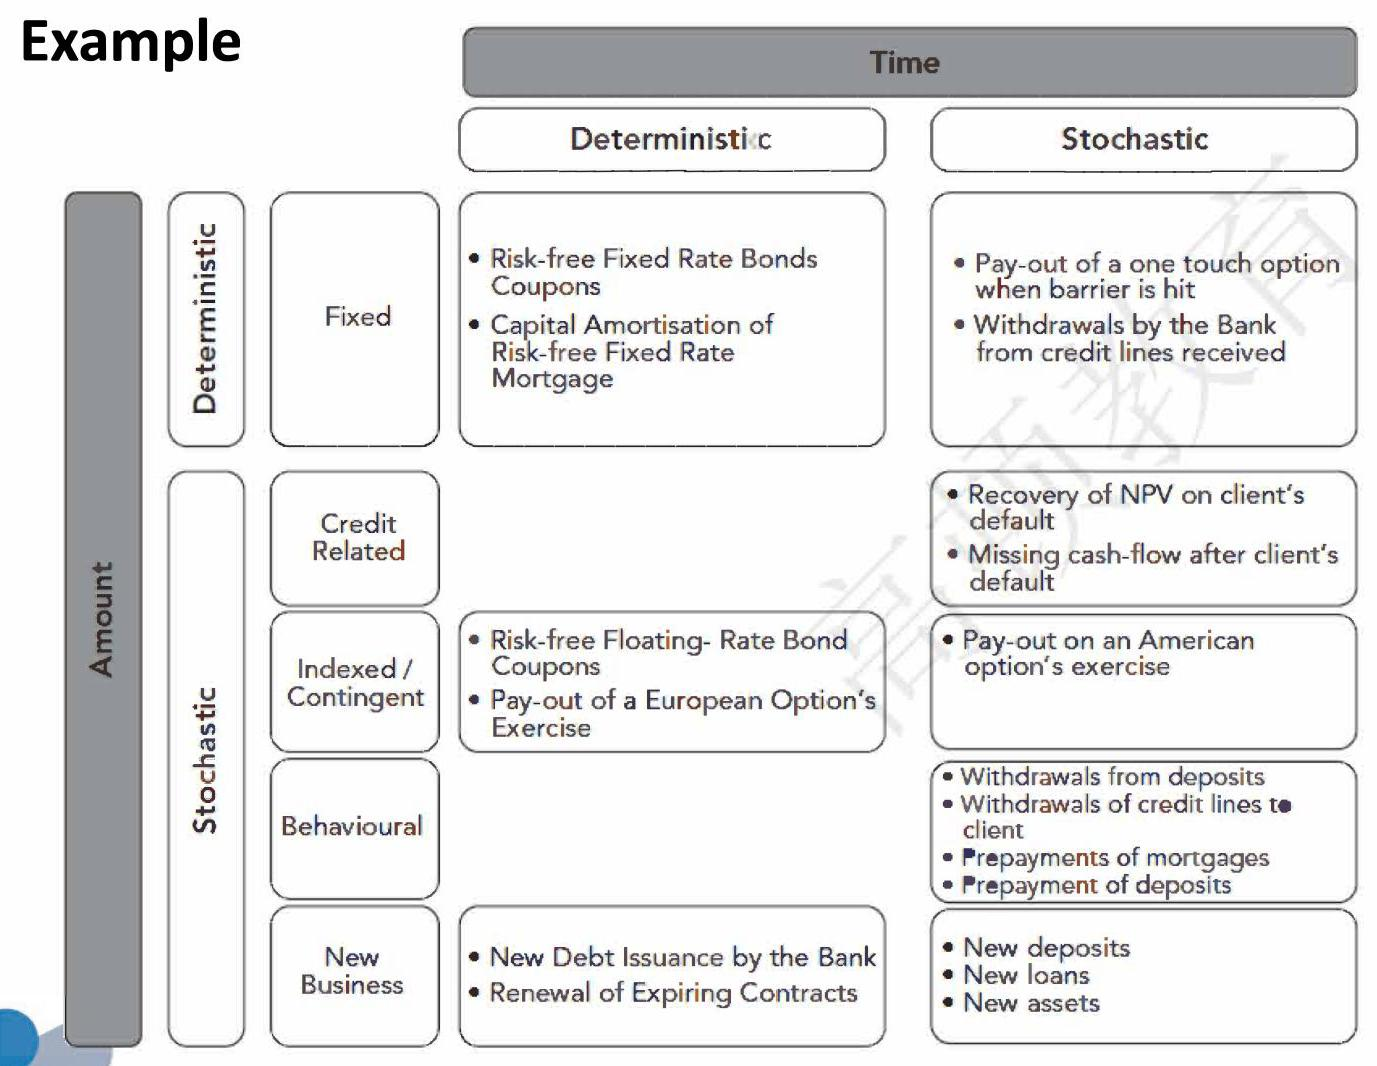
\includegraphics[width=0.5\textwidth]{images/taxonomy.jpg}
        \caption{taxonomy}
        \label{fig:labe22}
        \end{figure}
\end{itemize}




\subsubsection{Term structure of expected cash flows (TSECF):}
\begin{itemize}
\item Definition: TSECF can be defined as the collection, ordered by date, of expected cash flows, up to expiry referring to the contract with the longest maturity.
\end{itemize}

\subsubsection{Term structure of expected cumulated cash flows (TSECCF):}
\begin{itemize}
  \item Definition: TSECCF is the collection of expected cumulated cash flows ordered by date:
    \begin{itemize}
    \item Represents how the past dynamic evolution of net cash flows affects its total cash position on that date.
    \end{itemize}
\end{itemize}

\subsubsection{Example: TSECF \& TSECCF}
\begin{itemize}
  \item Consider a bank with a simplified balance sheet below:
  
  \begin{tabular}{lc|lc}
    Asset &  & Liability &  \\
    bonds & 30 & bonds & 40 \\
    loans & 70 & deposits & 40 \\
    \multicolumn{2}{c|}{} & Equity &  \\
    \multicolumn{2}{c|}{} & equity & 20
    \end{tabular}
  \item One key step to build the TSECF is to order the assets and the liabilities according to their maturity.
  
  \begin{center} % center环境使内部内容居中
    \begin{tabular}{|c|c|c|}
    \hline
    Time & Asset $cf_e^+$  & Liabilities  $cf_e^-$\\
    \hline
    1 & 20 &  \\
    2 &  & -10 \\
    3 &  &  \\
    4 &  &  \\
    5 & 50 &  \\
    6 &  &  \\
    7 &  & -70 \\
    8 &  &  \\
    9 &  &  \\
    10 & 30 &  \\
    $>10$ &  & -20 \\
    \hline
    \end{tabular}
\end{center}

  \item Table below shows a very simple balance sheet producing a very simple TSECF and related TSECCF.
  
  \begin{figure}[H]
    \centering
    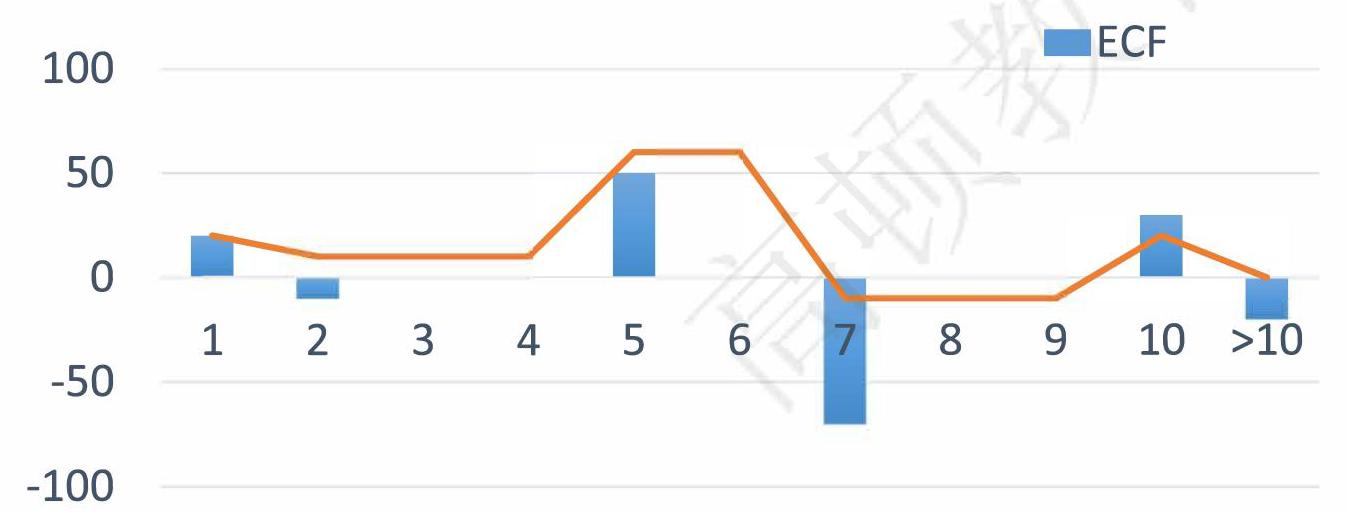
\includegraphics[width=0.5\textwidth]{images/ECF.jpg}
    \caption{ECF}
    \label{fig:labe22}
    \end{figure}
  \item Negative values in TESCCF: on an expected basis, this means the bank may become insolvent and eventually go bankrupt.
\end{itemize}

\subsubsection{Liquidity generation capacity (LGC)}
\begin{itemize}
\item Definition: LGC is the main tool a bank can use to handle the negative entries of the TSECCF.
    \begin{itemize}
    \item The ability of a bank to generate positive cash flows, beyond contractual ones, from the sources of liquidity available in/off the balance sheet at a given date.
    \end{itemize}
\item Three types of sources of liquidity:
    \begin{itemize}
    \item Selling of Assets (AS)
    \item Secured funding using assets as collateral
        \begin{itemize}
        \item Repo transactions (RP)
        \end{itemize}
    
    \item Unsecured funding (USF)
        \begin{itemize}
        \item Withdrawals of committed credit lines available from other financial institutions
        \item Deposit transactions in the interbank market
        \end{itemize}
    \end{itemize}
\end{itemize}




\subsubsection{The term structure of LGC (TSLGC)}
\begin{itemize}
  \item Definition: TSLGC as the collection of liquidity that can be generated at a given time, by the sources of liquidity, at the reference time up to a terminal time.
\end{itemize}


\subsubsection{Example: TSLGC \& TECLGC}

\begin{minipage}[c]{0.5\textwidth}
    \centering
    \begin{tabular}{|c|c|c|c|c|c|}
        \hline
        Time & AS & RP & USF & LGC & CLGC \\
        \hline
        1 & 0 & 0 & 0 & 0 & 0 \\
        2 & 0 & 0 & 0 & 0 & 0 \\
        3 & 0 & 0 & 0 & 0 & 0 \\
        4 & 0 & 0 & 0 & 0 & 0 \\
        5 & 0 & 0 & 0 & 0 & 0 \\
        6 & 0 & 0 & 0 & 0 & 0 \\
        7 & 2 & 5 & 3 & 10 & 10 \\
        8 & 1 & 2 & 1 & 4 & 14 \\
        9 & -0.5 & -1.5 & -0.5 & -2.5 & 11.5 \\
        10 & -2.5 & -5.5 & -3.5 & -11.5 & 0 \\
        $>10$ & 0 & 0 & 0 & 0 & 0 \\
        \hline
    \end{tabular}
\end{minipage}
\hfill
\begin{minipage}[c]{0.5\textwidth}
    \centering
    
\includegraphics[width=\textwidth]{LGC.jpg}
    \captionof{figure}{fig 21: LGC}
\end{minipage}


\subsubsection{The term structure of expected liquidity (\(\mathrm{TSL}_e\))}
\begin{itemize}
\item Definition: \(\mathrm{TSL}_e\) is basically a combination of the TSECCF and the TSCLGC.
    \begin{itemize}
    \item \(\mathrm{TSL}_e\) is in practice a measure to check whether the financial institution is able to cover negative cumulated cash flows at any time in the future, calculated at the reference date.
    \item  \(\mathrm{TSL}_e\) represents the main monitoring tool of a Treasury Department.
    \end{itemize}
\end{itemize}




\subsubsection{Example: \(\mathrm{TSL}_e\)}




\begin{minipage}[c]{0.45\textwidth}
    \centering
    \begin{tabular}{|c|c|c|c|}
        \hline
        Time & TSECCF & TSCLGC & TSLe \\
        \hline
        1 & 20 & 0 & 20 \\
        2 & 10 & 0 & 10 \\
        3 & 10 & 0 & 10 \\
        4 & 10 & 0 & 10 \\
        5 & 60 & 0 & 60 \\
        6 & 60 & 0 & 60 \\
        7 & -10 & 10 & 0 \\
        8 & -10 & 14 & 4 \\
        9 & -10 & 11.5 & 1.5 \\
        10 & 20 & 0 & 20 \\
        $>10$ & 0 & 0 & 0 \\
        \hline
        \end{tabular}
\end{minipage}
\hfill
\begin{minipage}[c]{0.45\textwidth}
    \centering
    
\includegraphics[width=\textwidth]{TSL.jpg}
    \captionof{figure}{fig 21: TSL}
\end{minipage}


\subsubsection{The term structure of available assets (TSAA)}
\begin{itemize}
\item Definition: TSAA is a tool used to monitor a bank's LGC and to provide an indication of the extent to which an asset can be used to create liquidity.
    \begin{itemize}
    \item Only shows how many single securities are available for inclusion in LGC.
        \begin{itemize}
        \item Does not imply that the notional amount of securities can be fully converted into liquidity.
        \end{itemize}
    \end{itemize}
\end{itemize}

\subsubsection{Transactions affect TESCF/TSAA/TSLGC}

\begin{table}[h]
    \centering
    \caption{Transaction Types and Their Impact on Liquidity Monitoring}
    \label{tab:transactions}
    \begin{tabular}{l|l|l|l|l|l}
    \toprule
    & & & \multicolumn{3}{c}{\textbf{Changes to}} \\
    \textbf{Type} & \textbf{Ownership} & \textbf{Possession} & \textbf{TSECF} & \textbf{TSAA} & \textbf{TSLGC} \\
    \midrule
    Buy & Bank & Bank & Yes & + & Possible \\
    Sell & Others & Others & Yes & - & Yes \\
    Repo & Bank & Others & No & - & Yes \\
    Reverse Repo & Others & Bank & Yes & + & Possible \\
    Sell/Buyback & Others & Others & Yes & - & Yes \\
    Buy/Sellback & Bank & Bank & Yes & + & Possible \\
    Security Lending & Bank & Others & Yes & - & No \\
    Security Borrowing & Others & Bank & Yes & + & Possible \\
    \bottomrule
    \end{tabular}
    \end{table}




\subsubsection{Cash flows at risk (cfaR):}
\begin{itemize}
  \item Cash flows are stochastic: not only the expected value but also its volatility.
  \item Cash flows at risk: showing the extreme values that both positive and negative cash flows assume during the time of their occurrence.
  \item Positive cash flow at risk :
    \[\mathrm{cfaR}^+_{\alpha}(t_0, t_i) = \mathrm{cf}^+_{\alpha}(t_0, t_i; x) - \mathbb{E}[\mathrm{cf}(t_0, t_i; x)]\]
  \item Negative cash flow at risk :
\[\mathrm{cfaR}^-_{1 - \alpha}(t_0, t_i) = \mathrm{cf}^-_{1 - \alpha}(t_0, t_i; x) - \mathbb{E}[\mathrm{cf}(t_0, t_i; x)]\]
    \begin{itemize}
    \item x: risk factors such as credit, behavioral and market variables e.g. interest rate
    \item $\alpha$: confidence level e.g. $\alpha$ = 99\%
    \end{itemize}


  \item Term structure of unexpected positive cash flows:
  \[
\mathrm{TSCF}^+_{\alpha}(t_0, t_b) = \left\{ \mathrm{cfaR}^+_{\alpha}(t_0, t_0), \mathrm{cfaR}^+_{\alpha}(t_0, t_1), \dots \mathrm{cfaR}^+_{\alpha}(t_0, t_b) \right\}
\]
    \begin{itemize}
    \item Upper bound of TESCF
    \end{itemize}
  \item Term structure of unexpected negative cash flows:
  \[
\mathrm{TSCF}^-_{1 - \alpha}(t_0, t_b) = \left\{ \mathrm{cfaR}^-_{1 - \alpha}(t_0, t_0), \mathrm{cfaR}^-_{1 - \alpha}(t_0, t_1), \dots \mathrm{cfaR}^-_{1 - \alpha}(t_0, t_b) \right\}
\]
    \begin{itemize}
    \item Lower bound of TESCF
    \end{itemize}
  \item Example: Maximum, minimum ( $\alpha$  = 99\%) and expected cash flows for a period of 20 days
  \begin{figure}[H]
    \centering
    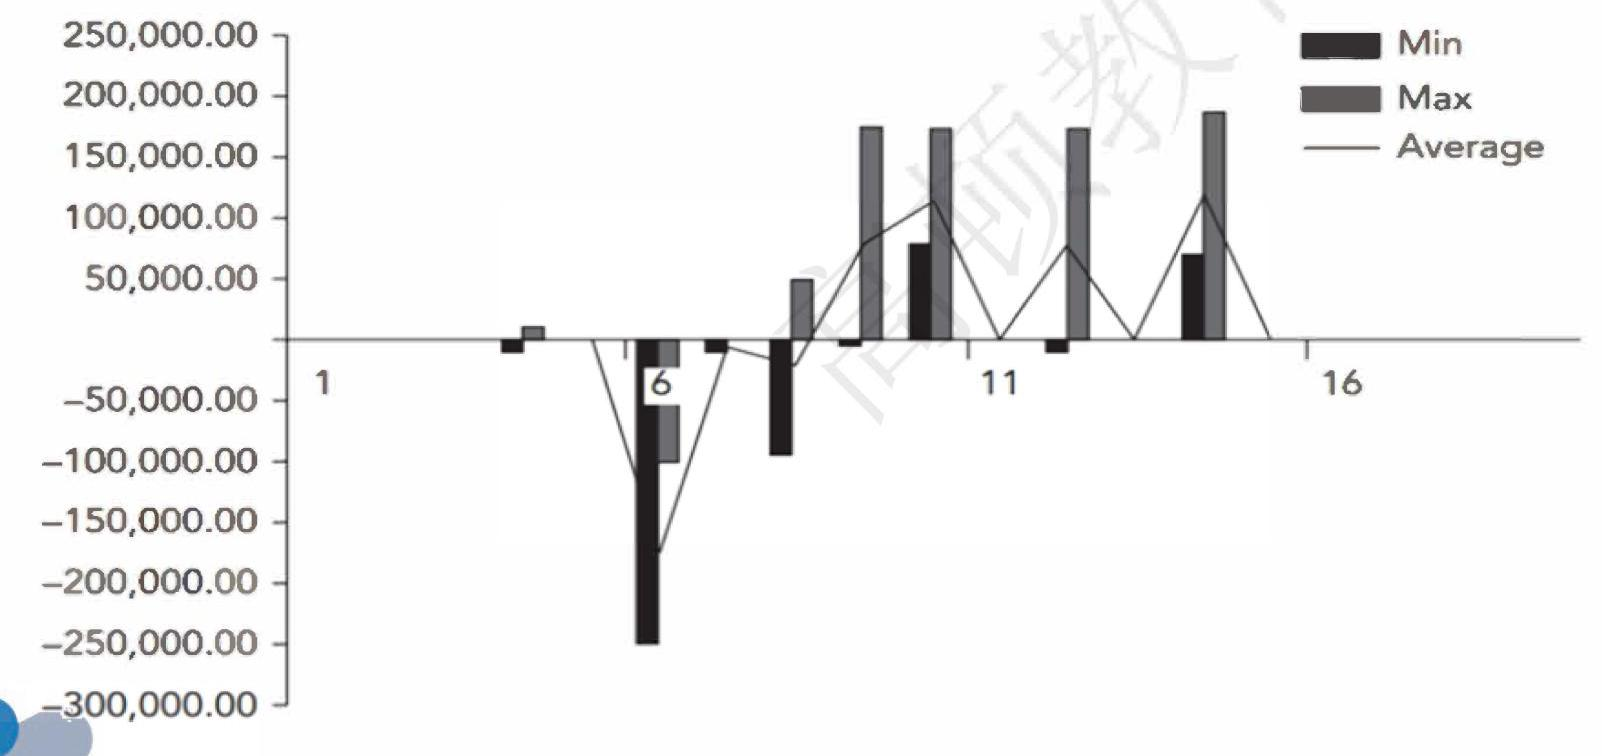
\includegraphics[width=0.5\textwidth]{images/CFAR.jpg}
    \caption{CFAR}
    \label{fig:labe22}
    \end{figure}
\end{itemize}

\subsubsection{Monitoring liquidity framework summary}
\begin{figure}[H]
    \centering
    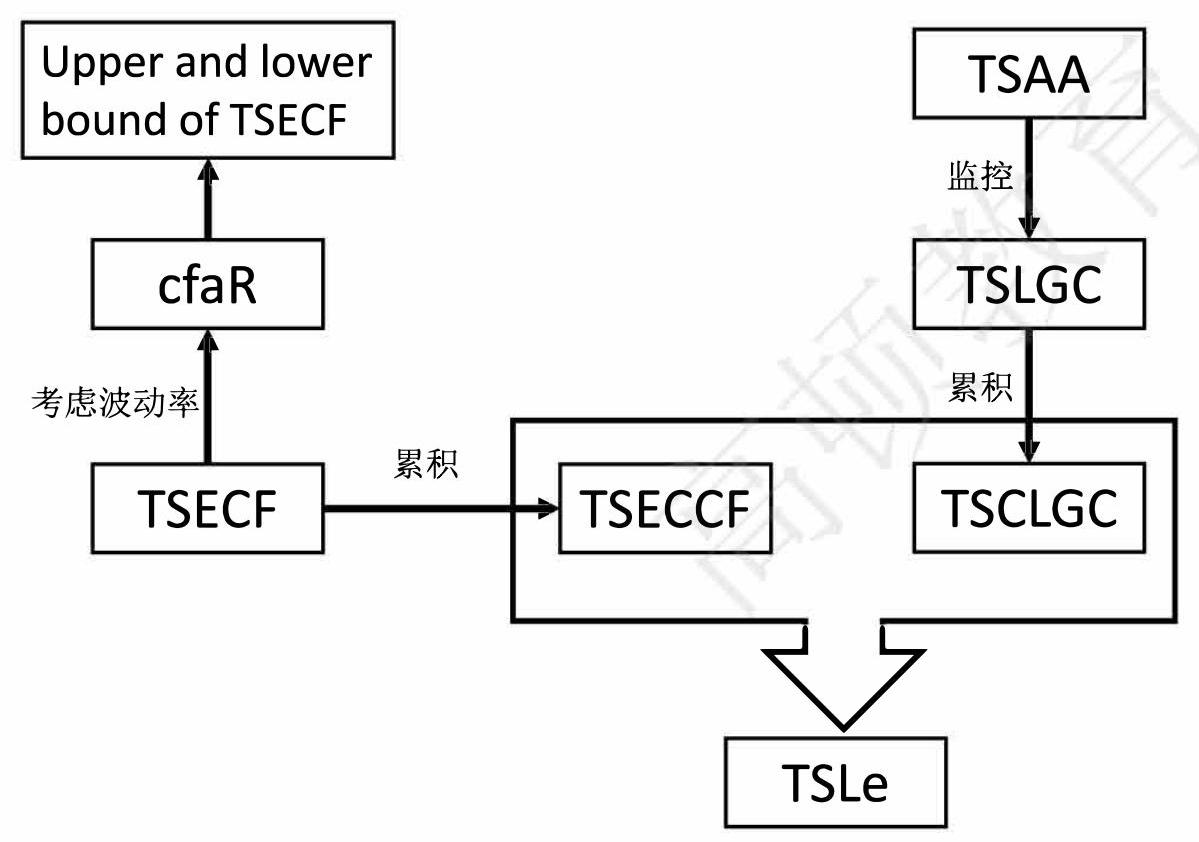
\includegraphics[width=0.5\textwidth]{images/TSLe.jpg}
    \caption{TSLe}
    \label{fig:labe22}
    \end{figure}




\subsection{Liquidity Transfer Pricing: A Guide Better Practice Ch15}





\subsubsection{Introduction of LTP}
\begin{itemize}
\item Liquidity Transfer Pricing (LTP) is a process that attributes the costs, benefits, and risks of liquidity to respective business units within a bank.
    \begin{itemize}
    \item Purpose of LTP:
        \begin{itemize}
        \item Transfer liquidity costs and benefits from business units to a centrally managed pool.
        \item Recoup the cost of carrying a liquidity cushion by charging contingent commitments.
        \end{itemize}
    \end{itemize}
\end{itemize}

\subsubsection{Process of LTP}

\begin{center}
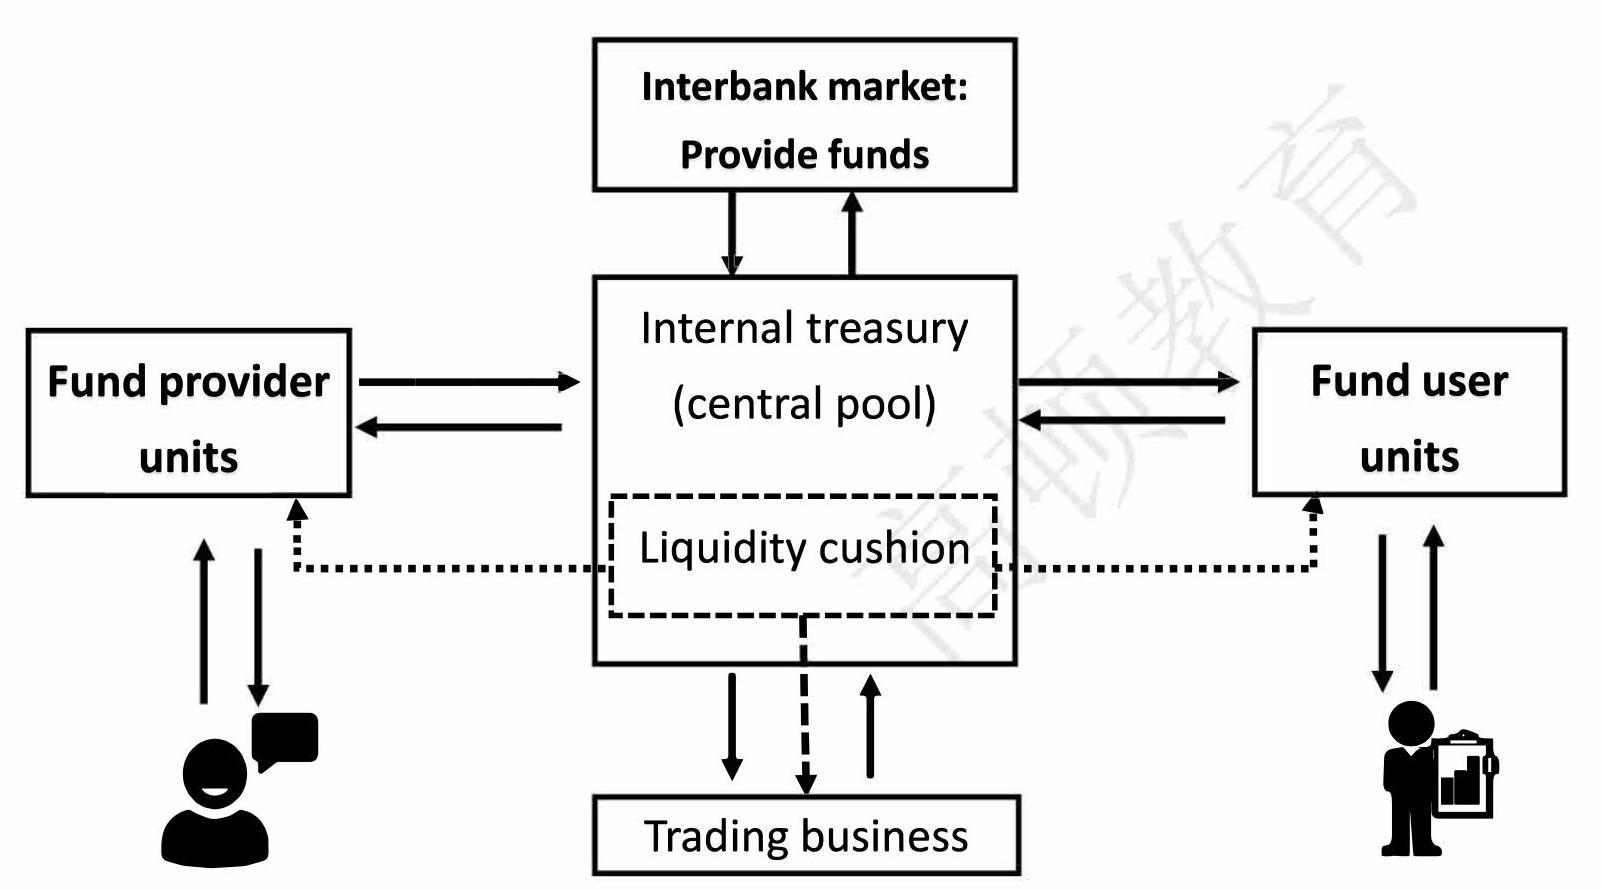
\includegraphics[width=0.9\textwidth]{images/0196c27c-0dc1-75f5-b50c-c29664ed0094_65_35_294_1601_889_0.jpg}
\end{center}

\subsubsection{Best Practices for LTP Process}

\begin{itemize}
  \item Governance of the LTP process
  \item Best practice 1: establish adequate LTP policies and procedures.
  \item Best practice 2: better to have a centralized funding center. Wholesale funding should be confined to this function.
  \item Best practice 3: develop trading book policies and identify funding requirements.
  \item Best practice 4: set up an effective oversight of the LTP process by independent risk and financial control personnel.
  \item Best practice 5: improve risk-adjusted profit measures to prompt business units to consider the cost of liquidity as part of their decision to book certain assets.
  \item Best practice 6: related parties involved in the management of LTP should better understand the LTP process. 


\end{itemize}

\subsubsection{Challenges in LTP Implementation}

\begin{itemize}
  \item Difficult to maintain proper oversight to manage and monitor the LTP process.
  \item The Liquidity Management Information Systems (LMIS) are unable to attribute the costs, benefits, and risks of liquidity appropriately to respective businesses at a sufficiently granular level.
    \begin{itemize}
    \item LMIS are widely used by management as a primary source of measuring and monitoring the performance of businesses.
    \end{itemize}
\end{itemize}




\subsubsection{Approaches of LTP}

\begin{itemize}
  \item \textbf{Zero cost of funds:}
    \begin{itemize}
      \item Definition: View funding liquidity as free, and funding liquidity risk as zero. (in an easy funding condition)
        \begin{itemize}
        \item Assume interest rate risk is properly accounted for using the swap curve: a zero spread above the swap curve implies a zero charge for the cost of funding liquidity.
        \end{itemize}
      \item Evaluation: the worst practice
      \item Results: the hoarding of long-term highly illiquid assets
      \begin{itemize}
        \item Few long-term stable liabilities to meet funding demand.
        \end{itemize} 
    \end{itemize}
    \begin{figure}[H]
        \centering
        \includegraphics[width=0.5\textwidth]{images/zero.jpg}
        \caption{zero}
        \label{fig:labe22}
        \end{figure}

  \item \textbf{Average cost of funds:}
    \begin{itemize}
    \item Pooled "average" cost of funds
        \begin{itemize}
        \item Definition: All assets and liabilities irrespective of their maturity are charged the same rate for cost/benefits of liquidity.
            \begin{itemize}
            \item Average rate calculated are based on all existing funding sources.
            \end{itemize}
        \item Evaluation: better than zero cost of funds
        \end{itemize}
        \begin{figure}[H]
            \centering
            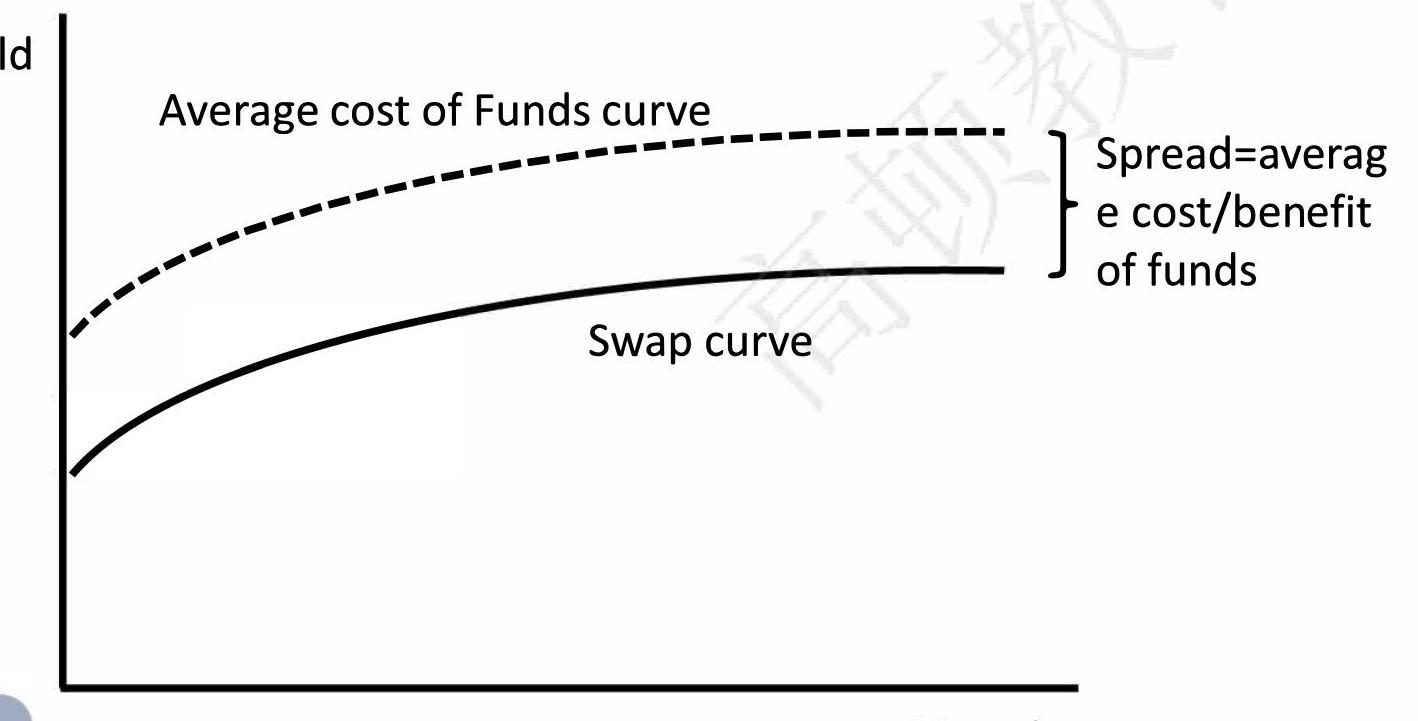
\includegraphics[width=0.5\textwidth]{images/Pooled.jpg}
            \caption{Pooled}
            \label{fig:labe22}
            \end{figure}

            \begin{table}[htbp]
                \centering
                \begin{tabular}{@{}lcccc@{}}
                \toprule
                Terms in years & 1 & 2 & 3 & 4 \\
                \midrule
                Loans/deposit principal & 1 million & 1 million & 1 million & 1 million \\
                Average cost of funds (bps) & 8 & 8 & 8 & 8 \\
                Charges for use of fund & 800 & 800 & 800 & 800 \\
                Credits for benefit of fund & 800 & 800 & 800 & 800 \\
                \bottomrule
                \end{tabular}
                \caption{Loan and Deposit - related Data}
                \label{tab:loan_deposit_data}
            \end{table}
    \item Separate "average" rates for cost and benefits of funds
        \begin{itemize}
        \item  Definition: average rates for cost of funds and benefits of fund are calculated separately.
            \begin{itemize}
            \item Loans can be encouraged or discouraged by adjusting  the average cost of using funds, without affecting the solicitation of funds by fund providers.
            \end{itemize}
        \item Evaluation: better than pooled "average" cost of funds
        \end{itemize}
        \begin{table}[htbp]
            \centering
            \begin{tabular}{@{}lcccc@{}}
            \toprule
            Terms in years & 1 & 2 & 3 & 4 \\
            \midrule
            Loans/deposit principal & 1 million & 1 million & 1 million & 1 million \\
            Average cost of funds (bps) & 8 & 8 & 8 & 8 \\
            Average benefit of funds (bps) & 3 & 3 & 3 & 3 \\
            Charges for use of fund & 800 & 800 & 800 & 800 \\
            Credits for benefit of fund & 300 & 300 & 300 & 300 \\
            \bottomrule
            \end{tabular}
            \caption{Financial Terms and Values}
            \label{tab:financial_data}
        \end{table}
    \item Results:
        \begin{itemize}
        \item Neglects the varying maturity of assets and liabilities by applying a single charge for the use and benefit of funds
        \item Lags changes in banks' actual market cost of funding.
        \item Promotes unhealthy maturity mismatch
        \item Distorts profit assessment
        \end{itemize}

    \end{itemize}
  \item \textbf{Matched-maturity marginal cost of funds:}
    \begin{itemize}
      \item Definition: using term liquidity premium to convert fixedrate borrowing costs to floating-rate borrowing costs through an internal swap transaction.
      \item Evaluation: current best practice but more complex than average cost
      
        \begin{figure}[H]
        \centering
        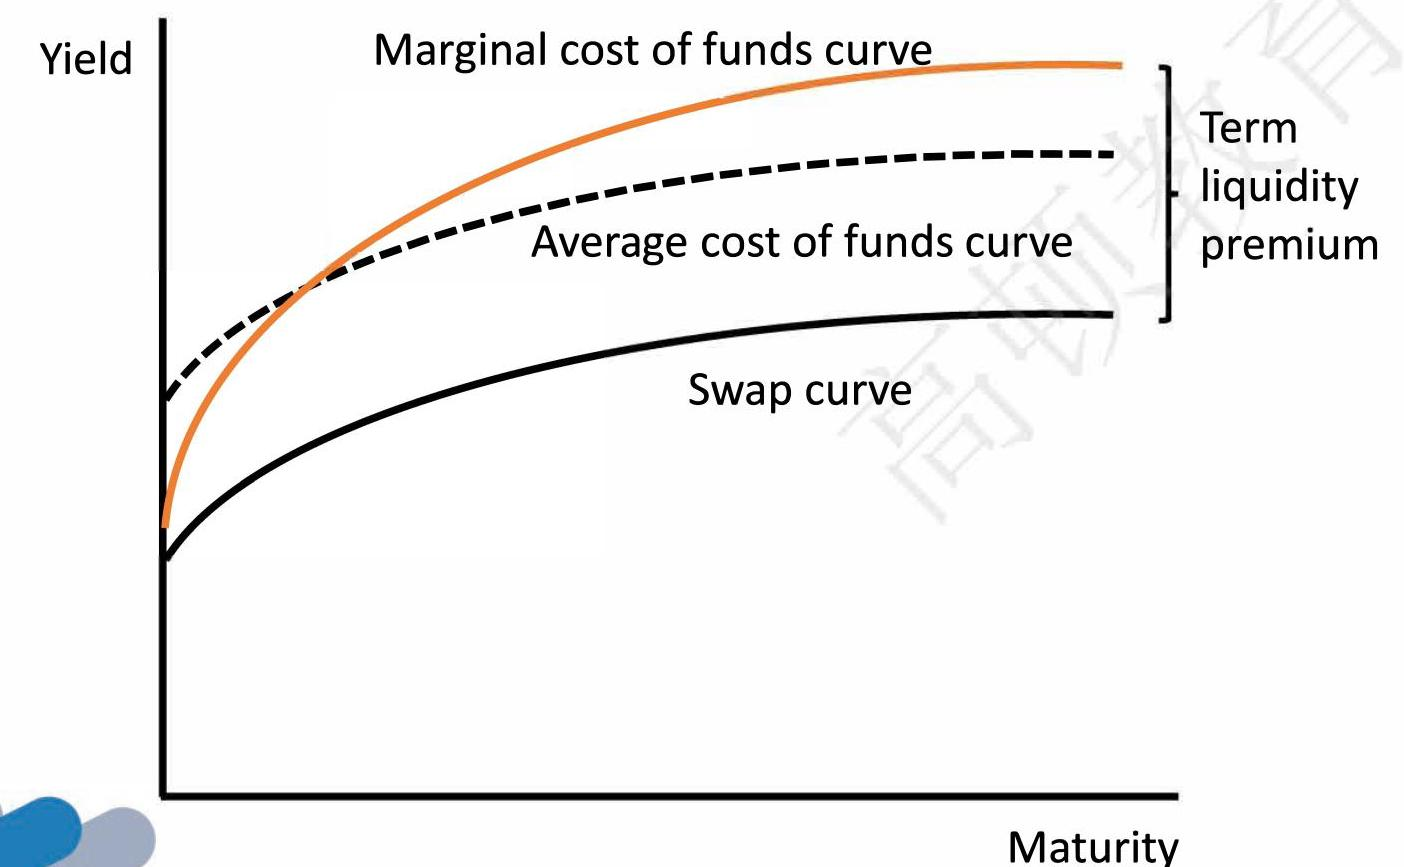
\includegraphics[width=0.5\textwidth]{images/Matched.jpg}
        \caption{Matched}
        \label{fig:labe22}
        \end{figure}
      

        \begin{table}[htbp]
            \centering
            \begin{tabular}{@{}lcccc@{}}
            \toprule
            Terms in years & 1 & 2 & 3 & 4 \\
            \midrule
            Term liquidity premium & 5 & 10 & 18 & 28 \\
            Average cost of funds (bps) & 8 & 8 & 8 & 8 \\
            \bottomrule
            \end{tabular}
            \caption{Liquidity and Cost Data}
            \label{tab:liquidity_cost_data}
        \end{table}

      \item Results:
        \begin{itemize}
        \item Recognize the costs and benefits of liquidity are related to the maturities of assets and liabilities.
            \begin{itemize}
            \item Assign higher rates to products that use or provide longer-term liquidity.
            \end{itemize}
        \item Recognize the importance of having changes in market conditions incorporated into the rate used to charge and credit users and providers of funds. (actual market cost)
        \end{itemize}
    \end{itemize}
\end{itemize}

\subsubsection{Contingent Liquidity Risk Pricing}

\begin{itemize}
  \item Contingent commitments may result in contingent liquidity risk.
    \begin{itemize}
    \item Lines of credit, collateral postings for derivatives and other financial contracts, etc.
    \end{itemize}
  \item Liquidity cushion: Banks carry a liquidity cushion, a buffer of highly liquid assets or stand-by liquidity to survive periods of unexpected funding outflows.
    \begin{itemize}
    \item Use the results of stress-testing to determine the size of the liquidity cushion.
    \end{itemize}
    
\end{itemize}





\subsubsection{Contingent liquidity risk pricing process}
\begin{itemize}
\item Process of Contingent liquidity risk pricing
    \begin{itemize}
    \item Step 1: Identify contingent commitments that are likely to create unexpected funding demands.
    \item Step 2: Perform stress tests under various scenarios to approximate the funding that might be required.
    \item Step 3: Net approximations from above against inflows generated.
        \begin{itemize}
        \item For example: through the sale of marketable securities to derive the size of the liquidity cushion.
        \end{itemize}
    \item Step 4: Calculate the cost of carry: the cost of funding liquid assets minus the return they generate.
    \item Step 5: Recoup cost of carry: charging a liquidity premium, at the most granular level, to the business unit, product or transaction that creates the need for the bank to carry such liquid assets.
    \end{itemize}
    
\end{itemize}


\subsubsection{Contingent liquidity risk pricing calculation}
\begin{itemize}
\item Method for pricing contingent liquidity risk in credit lines
    \begin{itemize}
    \item At the most basic level of what is considered to be better practice, all banks should be charging contingent commitments based on their likelihood of drawdown.
    \item Rate charge formular:
    \[
\frac{\text{limit} - \text{drawn amount}}{\text{limit}} \times \text{likelihood of drawdown} \times \text{cost funding liquidity cushion}
\]

    \item Example
        \begin{itemize}
        \item Suppose a line of credit with a limit of \$10 million has \$4 million already drawn. A 60 percent chance the customer will draw on the remaining credit and the cost of term funding assets in the liquidity cushion is 18 bps. Please calculate the rate cost of contingent liquidity risk.
        \end{itemize}
    \item Answer
        \[
\text{Dollar charge} = (\$10m - \$4m) \times 0.6 \times 0.0018 = 6480
\]
\[
\text{Rate charge} = \frac{6480}{\$10m} = 6.48 \text{bps}
\]

    \end{itemize}
\end{itemize}







\subsection{US dollar Shortage and Covered Interest Parity lost Ch 16 \& 17}


\subsubsection{Covered Interest Parity}

\begin{itemize}
  \item CIP is a no-arbitrage condition according to which interest rates on two otherwise identical assets in two different currencies should be equal once the foreign currency risk is hedged:
  \[\frac{F}{S} = \frac{1 + r}{1 + r^*}\]
    \begin{itemize}
    \item S: spot exchange rate in units of US dollar per foreign currency
    \item F: corresponding forward exchange rate
    \item r: the US dollar interest rate
    \item $r^*$: the foreign currency interest rate.
    \end{itemize}

  \item In practice, the relationship between \(F\) and \(S\) is observed in market transactions in FX instruments, notably FX swaps and cross-currency swaps.
\end{itemize}



\subsubsection{FX Swaps vs. Cross-currency Swaps}

\begin{itemize}
\item \textbf{Mechanics of FX swaps:}
      \begin{itemize}
        \item See diagram below.
        \item S: Spot exchange rate; F: predetermined forward exchange rate; X: Principal.
        \item Counterparty A: borrowing US dollar; Counterparty B: lending US dollar.
      \end{itemize}
      \begin{center}
      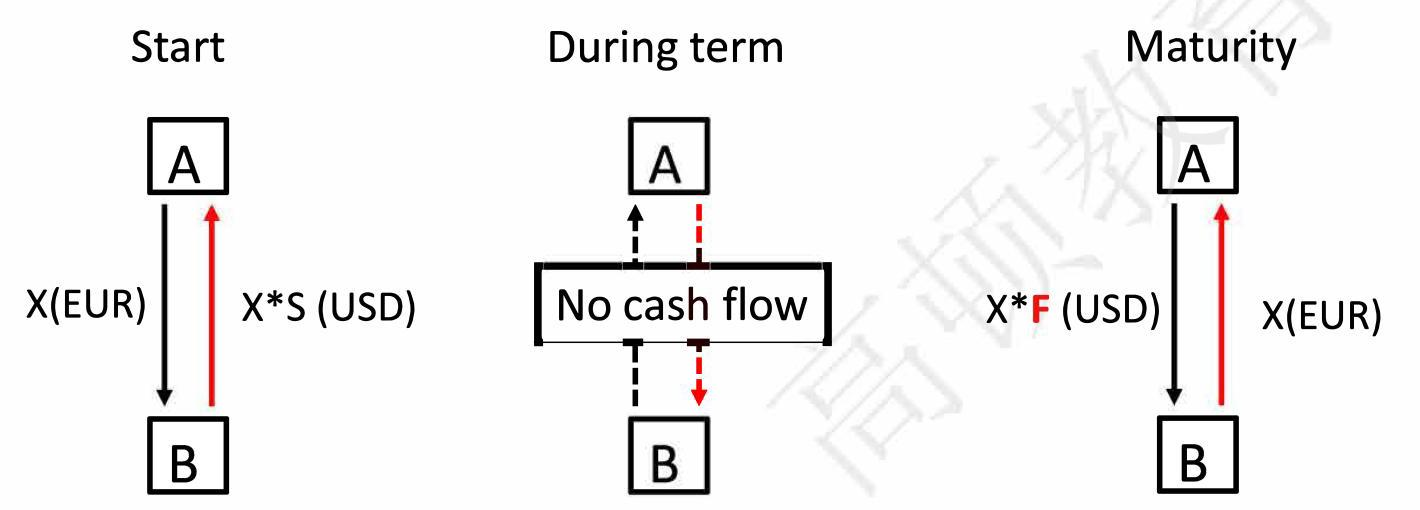
\includegraphics[width=0.8\textwidth]{images/0196c27c-0dc1-75f5-b50c-c29664ed0094_96_120_464_1420_510_0.jpg}
      \end{center}
      \begin{itemize}

      \item If \(b \neq 0\), the CIP fails: the party lending a currency via FX swaps makes a higher or lower return than implied by the interest rate differential in the two currencies.
      \[
      \frac{F}{S} = \frac{1 + {r}^{USD} + b}{1 + {r}^{foreign}}
      \]
    \end{itemize}

    \item \textbf{Mechanics of cross-currency swaps:}
      
      \begin{center}
      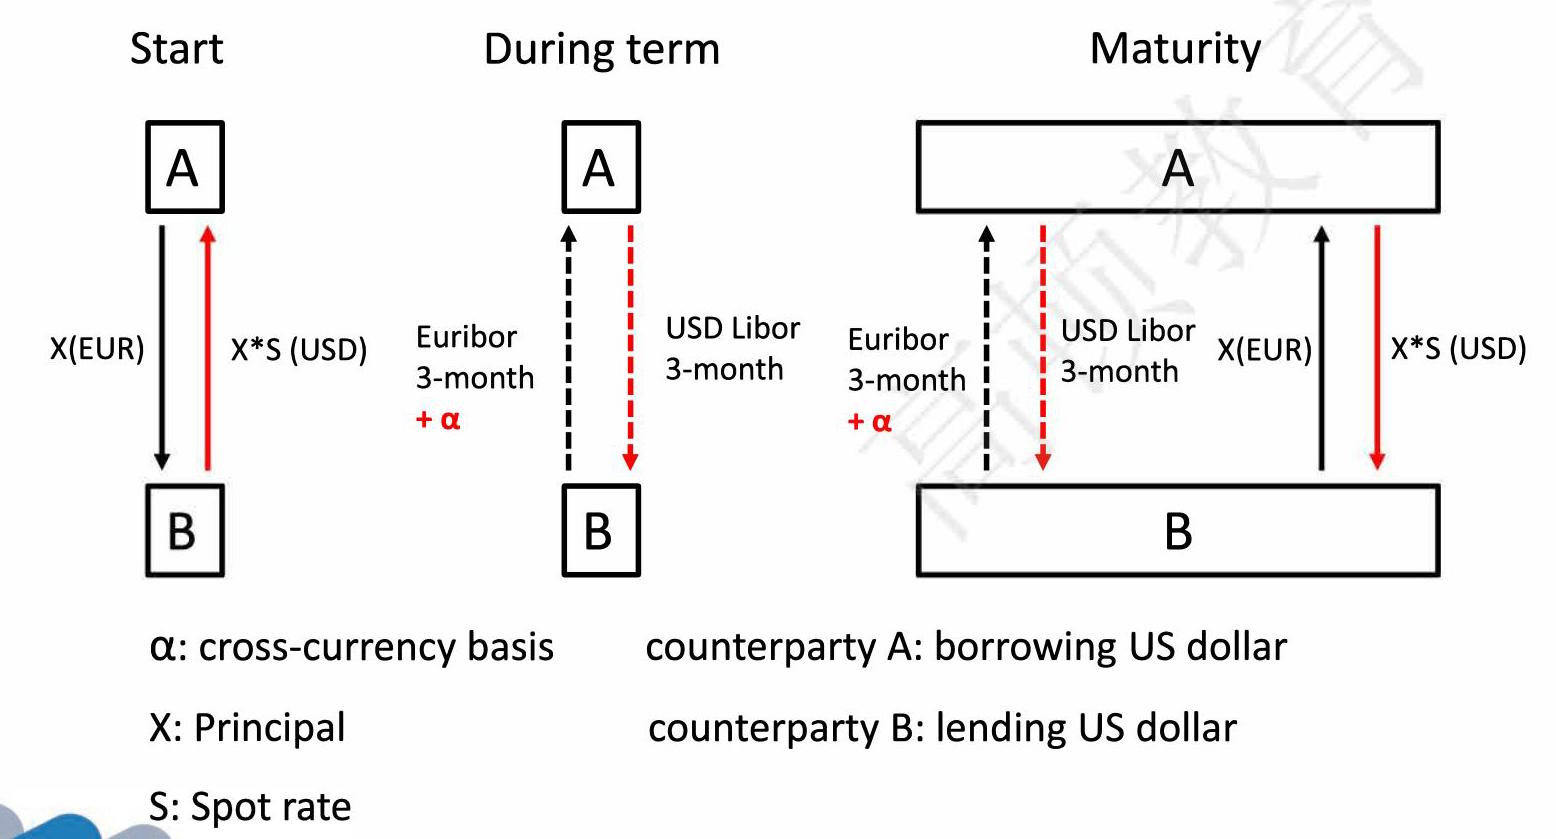
\includegraphics[width=0.9\textwidth]{images/0196c27c-0dc1-75f5-b50c-c29664ed0094_98_28_419_1556_839_0.jpg}
      \end{center}
      \begin{itemize}

      \item When \(\alpha \neq 0\), the failure of CIP if the party lending US dollars in a cross-currency swap pay the basis, non-zero \(\alpha\), on top of foreign currency.
      \item In a cross-currency basis swap, interest payments are based on the respective Libor rates plus the basis \(\alpha\).
  \end{itemize}
\end{itemize}








\subsubsection{Introduction of Cross-Currency Basis}
\begin{itemize}
\item Key factors affecting the cross-currency swap basis:
    \begin{itemize}
    \item Drop in market liquidity
        \begin{itemize}
        \item Market liquidity in the underlying instruments may evaporate, so that the difference between bid and ask prices for forward and spot transactions is non-trivial.
        \end{itemize}
    \item Risk increases of the underlying instruments
        \begin{itemize}
        \item For example, a rise in counterparty credit risks in the interbank markets
        \end{itemize}
    \end{itemize}
\end{itemize}


\subsubsection{The violation of CIP}
\begin{itemize}
\item Negative basis points period: Since 2007, the basis for lending US dollars against most currencies, notably the euro and yen, has been negative.
    \begin{itemize}
    \item Borrowing dollars through the swap market became more expensive than direct funding in the dollar cash market.
    \end{itemize}
\item Reflection of CIP violation: strains in global interbank markets.
    \begin{itemize}
    \item Counterparty risk
    \item Constrained bank access to wholesale dollar funding inhibited arbitrage
    \end{itemize}
\item Figure of XCCY ( \(\alpha\): cross-currency basis)
\begin{center}
    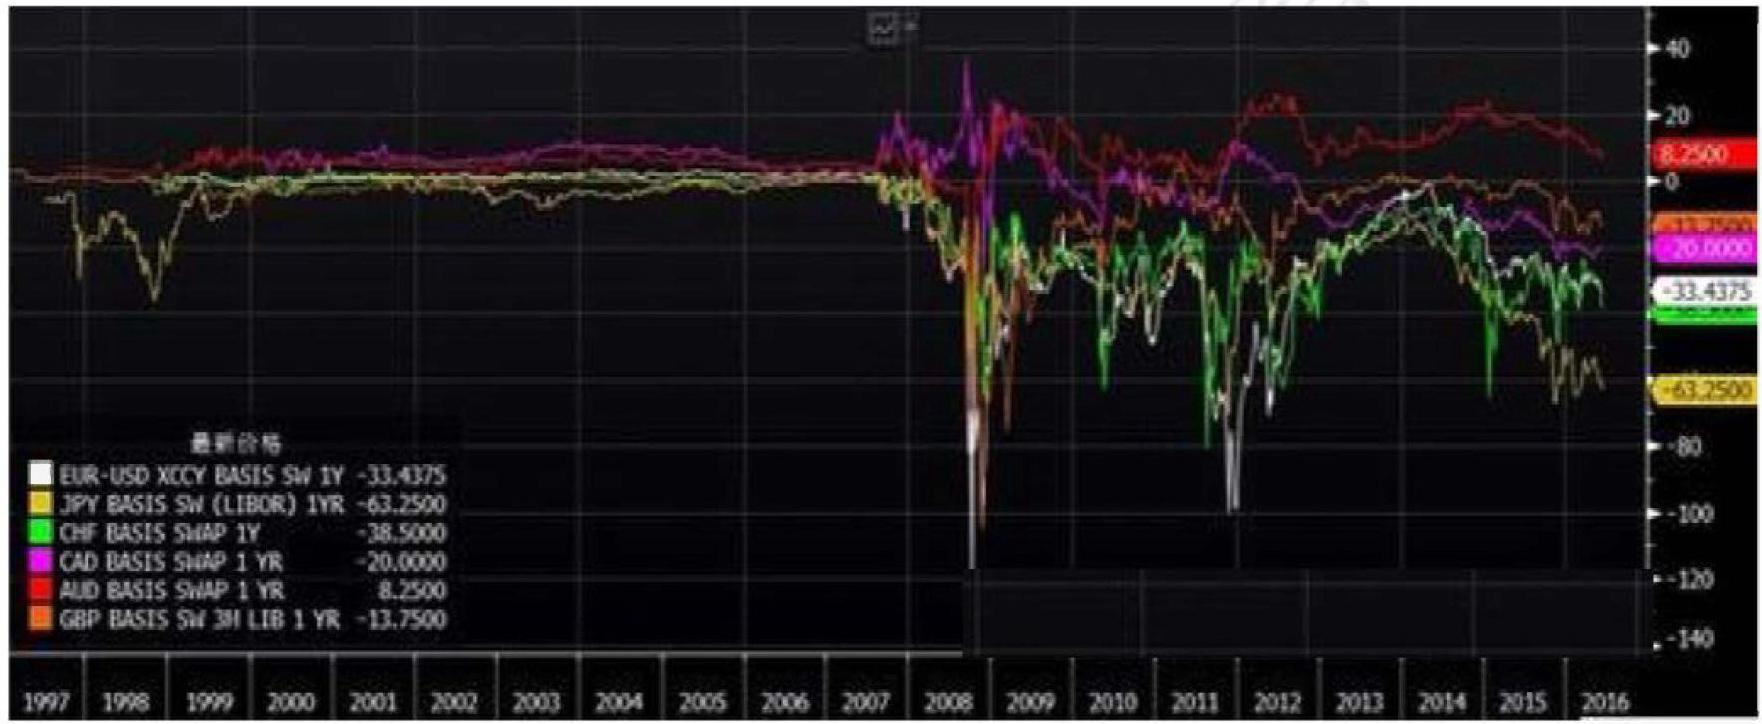
\includegraphics[width=0.9\textwidth]{images/XCCY.jpg}
    \end{center}
\end{itemize}


\subsubsection{Causes Of CIP Violation}
\begin{itemize}
\item Demand for currency hedges
    \begin{itemize}
    \item The reason of why the basis opens up
    \end{itemize}
\item New constraints on arbitrage activity
    \begin{itemize}
    \item The reason why the basis does not close
    \end{itemize}
\end{itemize}


\subsubsection{Demand for currency hedges}
\begin{itemize}
\item Three sources of hedging demand
    \begin{itemize}
    \item Demand from banks
        \begin{itemize}
        \item Foreign currency hedges from banks' business models
        \end{itemize}
    \item Demand from institutional investors
        \begin{itemize}
        \item Strategic hedging decisions of institutional investors
        \end{itemize}
    \item Demand from Non-financial firms
        \begin{itemize}
        \item Non-financial firms' debt issuance across currencies
        \end{itemize}
    \end{itemize}
\end{itemize}




\subsubsection{New constraints on arbitrage activity}
\begin{itemize}
\item Market structural changes tighten limits to arbitrage.
  \begin{itemize}
  \item Structural changes in how market participants have been pricing market, credit, counterparty and liquidity risks postcrisis have tightened limits to arbitrage.
  \end{itemize}
\item Balance sheet space is not free and arbitrage can be both costly and risky.
  \begin{itemize}
  \item Arbitrage enlarges its balance sheet, and banks possibly face credit risk, mark-to-market and liquidity risk.
  \end{itemize}
\item Changes in regulation have reinforced market pressures for a tighter management of balance sheet risks.
  \begin{itemize}
  \item Derivatives transaction changes: changes related to credit value adjustments have sought to incentivize dealers to price the counterparty risk more accurately
  \item Basel Ill and US leverage ratios changes: potential future exposure adjustment charges require market participants to hold capital in proportion to their derivatives and other exposures.
  \end{itemize}
\end{itemize}





\subsubsection{Background introduction}
\begin{itemize}
\item Introduction: Global banking activity had grown remarkably between 2000 and mid-2007. As bank's balance sheets expanded, they appetite for foreign currency assets like US dollar loans and structural products.
  \begin{itemize}
  \item Banks borrow US dollars to invest:
    \begin{itemize}
    \item Borrow domestic currency and convert to U.S. dollars in the spot market.
    \item Using FX swap convert domestic currency to US dollars
    \item Borrowing US dollar from interbank market.
    \end{itemize}
    
  \end{itemize}
\end{itemize}



\subsubsection{Maturity/currency transformation}
\begin{itemize}
\item US dollar maturity funding gap
  \begin{itemize}
  \item US dollar investment to non-banks are funded by liabilities to various counterparties with various maturities, subjected to considerable funding risk.
    \begin{itemize}
    \item The amount of US dollars invested in longer-term assets which is not supported by longer-term US dollars liabilities.
    \end{itemize}
    
  \item This gap must roll over before their investment mature.
  \end{itemize}
  
\end{itemize}



\subsubsection{Causes of the shortage of US dollars}
\begin{itemize}
\item Unsustainable maturity transform: The major sources of short-term funding turned out to be less stable than expected.
  \begin{itemize}
  \item FX swap became expensive: The heightened counterparty risk and liquidity concerns in FX swap markets made it even more expensive to obtain US dollars via currency swaps.
  \item Non-bank sources of funds is instable: Money market funds, facing large redemptions following the failure of Lehman Brothers, withdrew from bank-issued paper, threatening a wholesale run on banks.
  \item Market conditions during the crisis have made it difficult for banks to respond to funding pressures by reducing their US dollar assets: such as structured finance products, were harder to sell without realising large losses.
  \end{itemize}
\end{itemize}



\subsubsection{The international policy response}
\begin{itemize}
\item Temporary reciprocal currency arrangement (swap lines) between Federal Reserve and European central banks: The Federal Reserve channel US dollars to European central banks, then the European central banks channel to European banks in their respective jurisdictions unlimitedly.
\item Swap lines extended across continents to central banks in Australia and New Zealand, Scandinavia, and several countries in Asia and Latin America, forming a global network.
\item The advantages of the swap line between central banks:
  \begin{itemize}
  \item 央行具有货币发行权: Federal Reserve and its central bank counterparties have the power to create any amount of money, in contrast with international financial institutions administering limited resources.
  \item 无信息不对称引起的道德风险: Swap network does not compound the informational problems that can give rise to moral hazard.
  \end{itemize}
\end{itemize}


